




%----------------------------------------------------------------------------------------


%%%%%%%%%%%%%%%%%%%%%%%
\section{Quantitative Epistemology}{Epistémologie Quantitative}

\label{app:sec:quantepistemo}


%----------------------------------------------------------------------------------------

\subsection{Algorithmic systematic review}{Revue systématique algorithmique}

\paragraph{Implementation}{Implémentation}


\bpar{
Because of the heterogeneity of operations required by the algorithm (references organisation, catalog requests, text processing), it was found a reasonable choice to implement it in Java. Source code is available on the Github repository of the project\footnote{at \texttt{https://github.com/JusteRaimbault/CityNetwork/tree/master/Models/QuantEpsitemo/AlgoSR}}. Catalog request, consisting in retrieving a set of references from a set of keywords, is done using the Mendeley software API \cite{mendeley} as it allows an open access to a large database. Keyword extraction is done by Natural Language Processing (NLP) techniques, following the workflow given in \cite{chavalarias2013phylomemetic}, calling a Python script that uses \cite{bird2006nltk}.
}{
De par l'hétérogénéité des opérations requises par l'algorithme (organisation des références, requêtes au catalogue, analyse textuelle), le language Java s'est présenté comme une alternative raisonnable. Le code source est disponible sur le dépôt ouvert du projet\footnote{à l'adresse \texttt{https://github.com/JusteRaimbault/CityNetwork/tree/master/Models/QuantEpistemo/AlgoSR}}. Les requêtes au catalogue, qui consistent à récupérer un ensemble de références à partir d'un ensemble de mots-clés, sont faites via l'API du logiciel Mendeley~\cite{mendeley} qui permet un accès ouvert à une base de données conséquente. L'extraction des mots-clés est effectuée par techniques d'Analyse Textuelle (NLP) selon le processus donné dans~\cite{chavalarias2013phylomemetic}, via un script Python qui utilise~\cite{bird2006nltk}.
}


\paragraph{Convergence and Sensitivity Analysis}{Convergence et analyse de sensibilité}


\comment{(Florent) avec quels mots clés as tu validé empiriquement la convergence de l'algo?}

\bpar{
A formal proof of algorithm convergence is not possible as it will depend on the empirical unknown structure of request results and keywords extraction. We need thus to study empirically its behavior. Good convergence properties but various sensitivities to $N_k$ were found as presented in Fig.~\ref{fig:quantepistemo:sensitivity}. We also studied the internal lexical consistence of final corpuses as a function of keywords number. As expected, small number yields more consistent corpuses, but the variability when increasing stays reasonable.
}{
Une preuve formelle de convergence de l'algorithme n'est guère envisageable puisque qu'elle dépendra de la structure empirique inconnue des résultats de requête et d'extraction de mots-clés. Il est donc nécessaire d'étudier le comportement de l'algorithme de manière empirique. Comme présenté en figure~\ref{fig:quantepistemo:sensitivity}, l'algorithme a de bonnes propriétés de convergence mais diverse sensibilités à $N_k$. Nous étudions également la cohérence lexicale interne des corpus finaux et fonction du nombre de mots-clés. Comme attendu, des valeurs faibles produisent des corpus plus cohérents, mais la variabilité lorsque qu'elles augmentent reste raisonnable.
}



%%%%%%%%%%%%%%%%%%%%%%%%%%%%
\begin{figure}
\centering
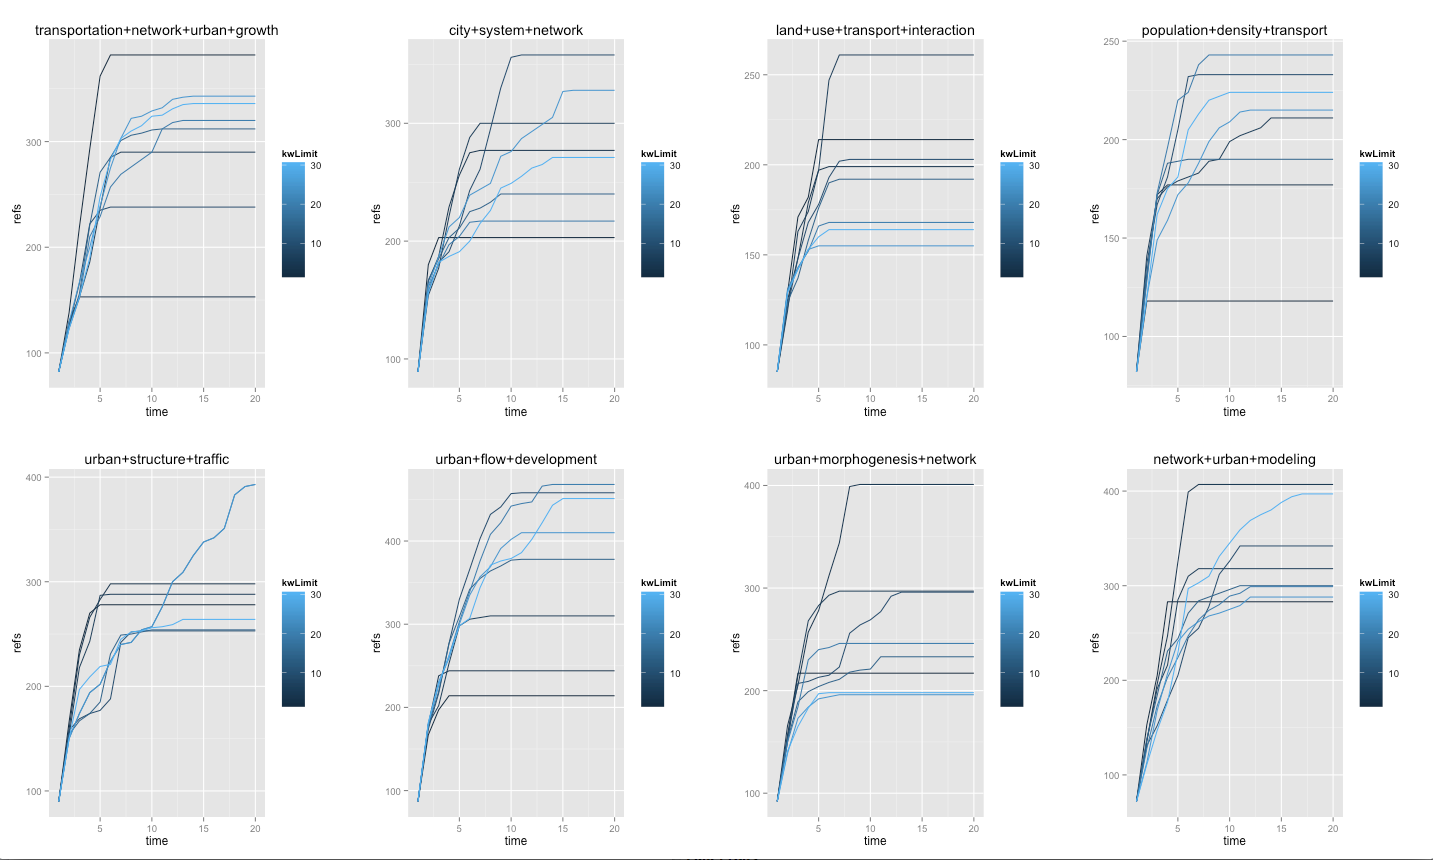
\includegraphics[width=\textwidth]{Figures/QuantEpistemo/explo} % Convergence and sensitivity analysis of systematic review algorithm
\medskip
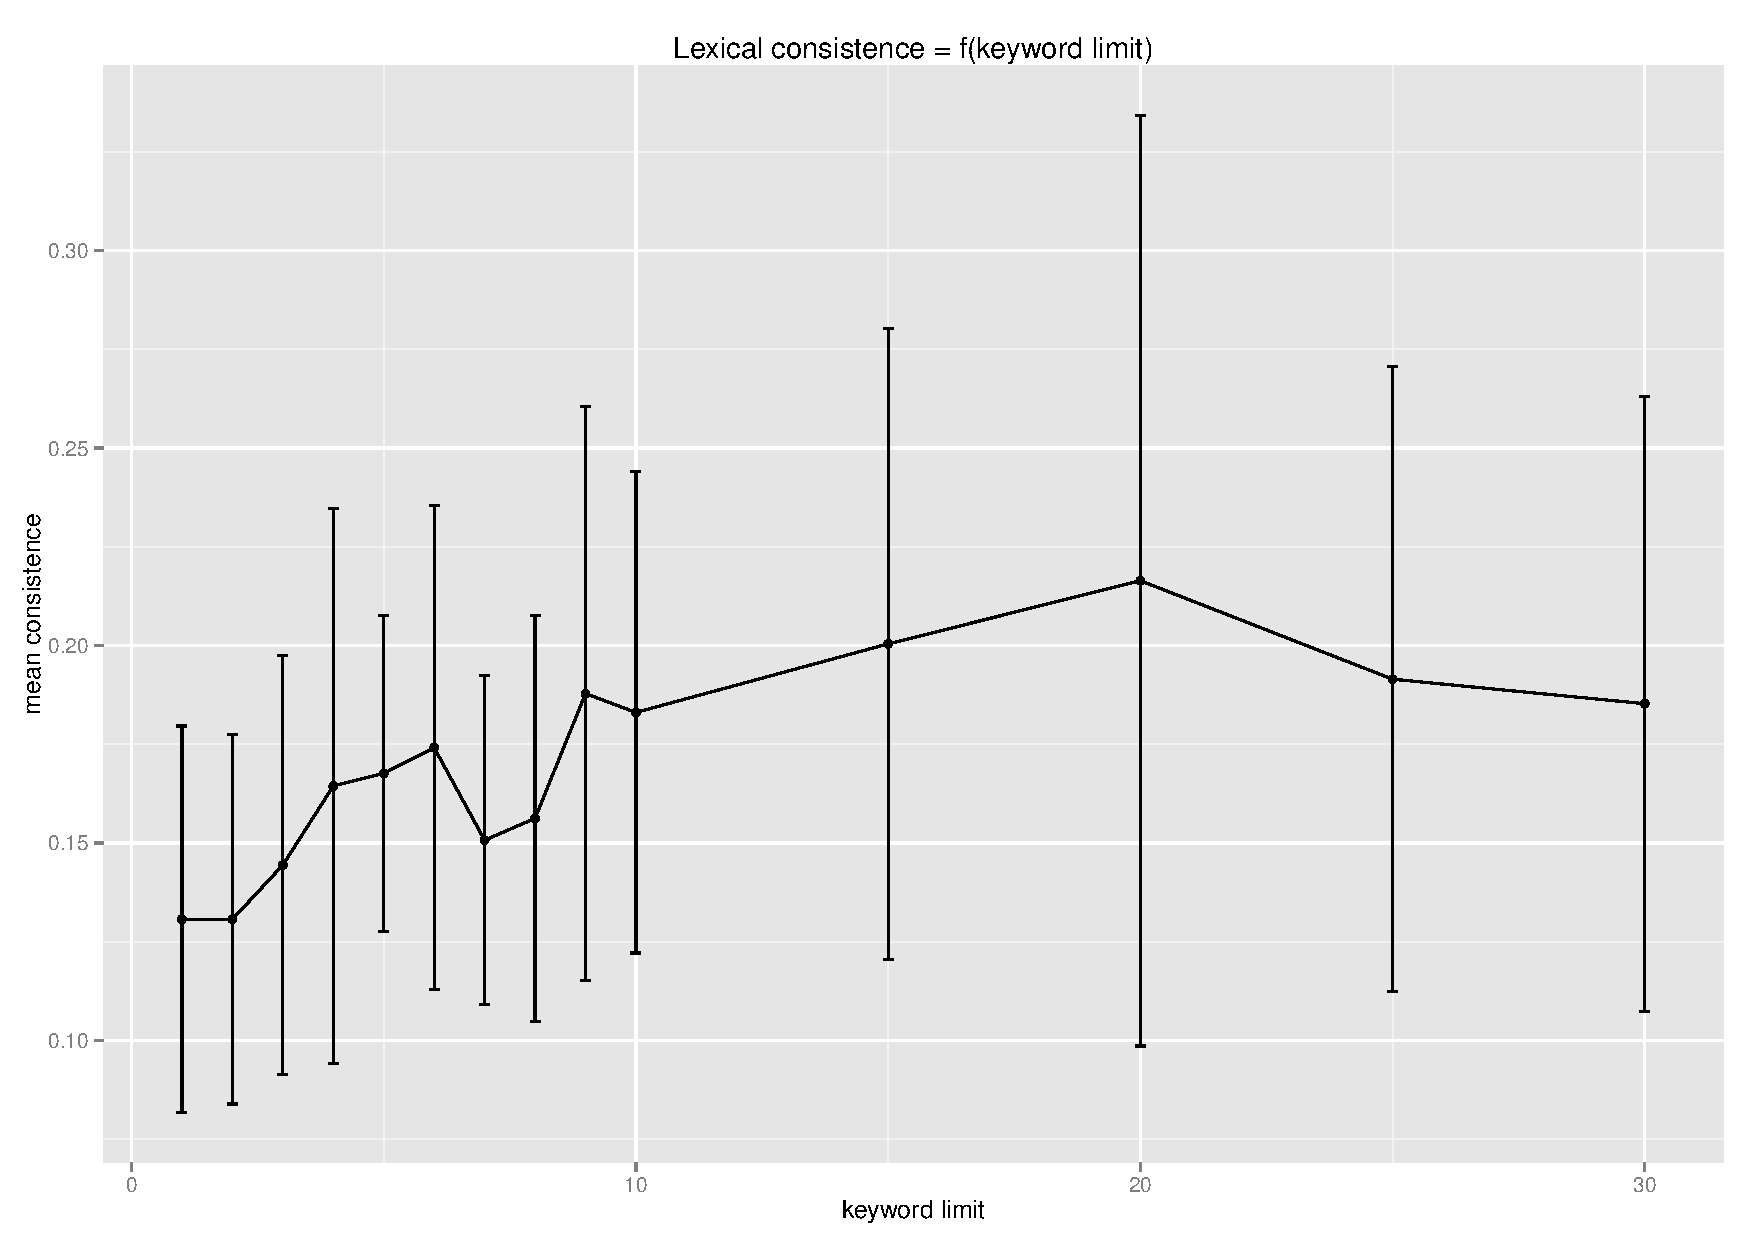
\includegraphics[width=0.8\textwidth]{Figures/QuantEpistemo/lexicalConsistence_MeanSd}
\caption[][]{Convergence and sensitivity analysis. Left : Plots of number of references as a function of iteration, for various queries linked to our theme (see further), for various values of $N_k$ (from 2 to 30). We obtain a rapid convergence for most cases, around 10 iterations needed. Final number of references appears to be very sensitive to keyword number depending on queries, what seems logical since encountered landscape should strongly vary depending on terms. Right : Mean lexical consistence and standard error bars for various queries, as a function of keyword number. Lexical consistence is defined though co-occurrences of keywords by, with $N$ final number of keywords, $f$ final step, and $c(i)$ co-occurrences in references, $k = \frac{2}{N(N-1)}\cdot \sum_{i,j \in \mathcal{K}_f}{\left| c(i) - c(j) \right|}$. The stability confirms the consistence of final corpuses.}{\comment{(Florent) illisible}}
\label{fig:quantepistemo:sensitivity}
\end{figure}
%%%%%%%%%%%%%%%%%%%%%%%%%%%%











%----------------------------------------------------------------------------------------

\subsection{Hypernetwork analysis}{Analyse par hyperréseau}


\paragraph{Initial corpus}{Corpus initial}


Le tableau~\ref{tab:app:quantepistemo:corpus} donne la composition du corpus par domaines.

%\begin{table}
% a completer
%\caption{}{}
%\label{tab:app:quantepistemo:corpus}
%\end{table}





\paragraph{Sensitivity analysis}{Analyse de sensibilité}

L'analyse de sensibilité permettant de fixer les paramètres optimaux pour le réseau sémantique est montrée en Fig.~\ref{fig:app:quantepistemo:sensitivity}.

% degré non pondéré ? -> justifié dans le Cybergeo paper


%%%%%%%%%%%%%%%%%%
\begin{figure}
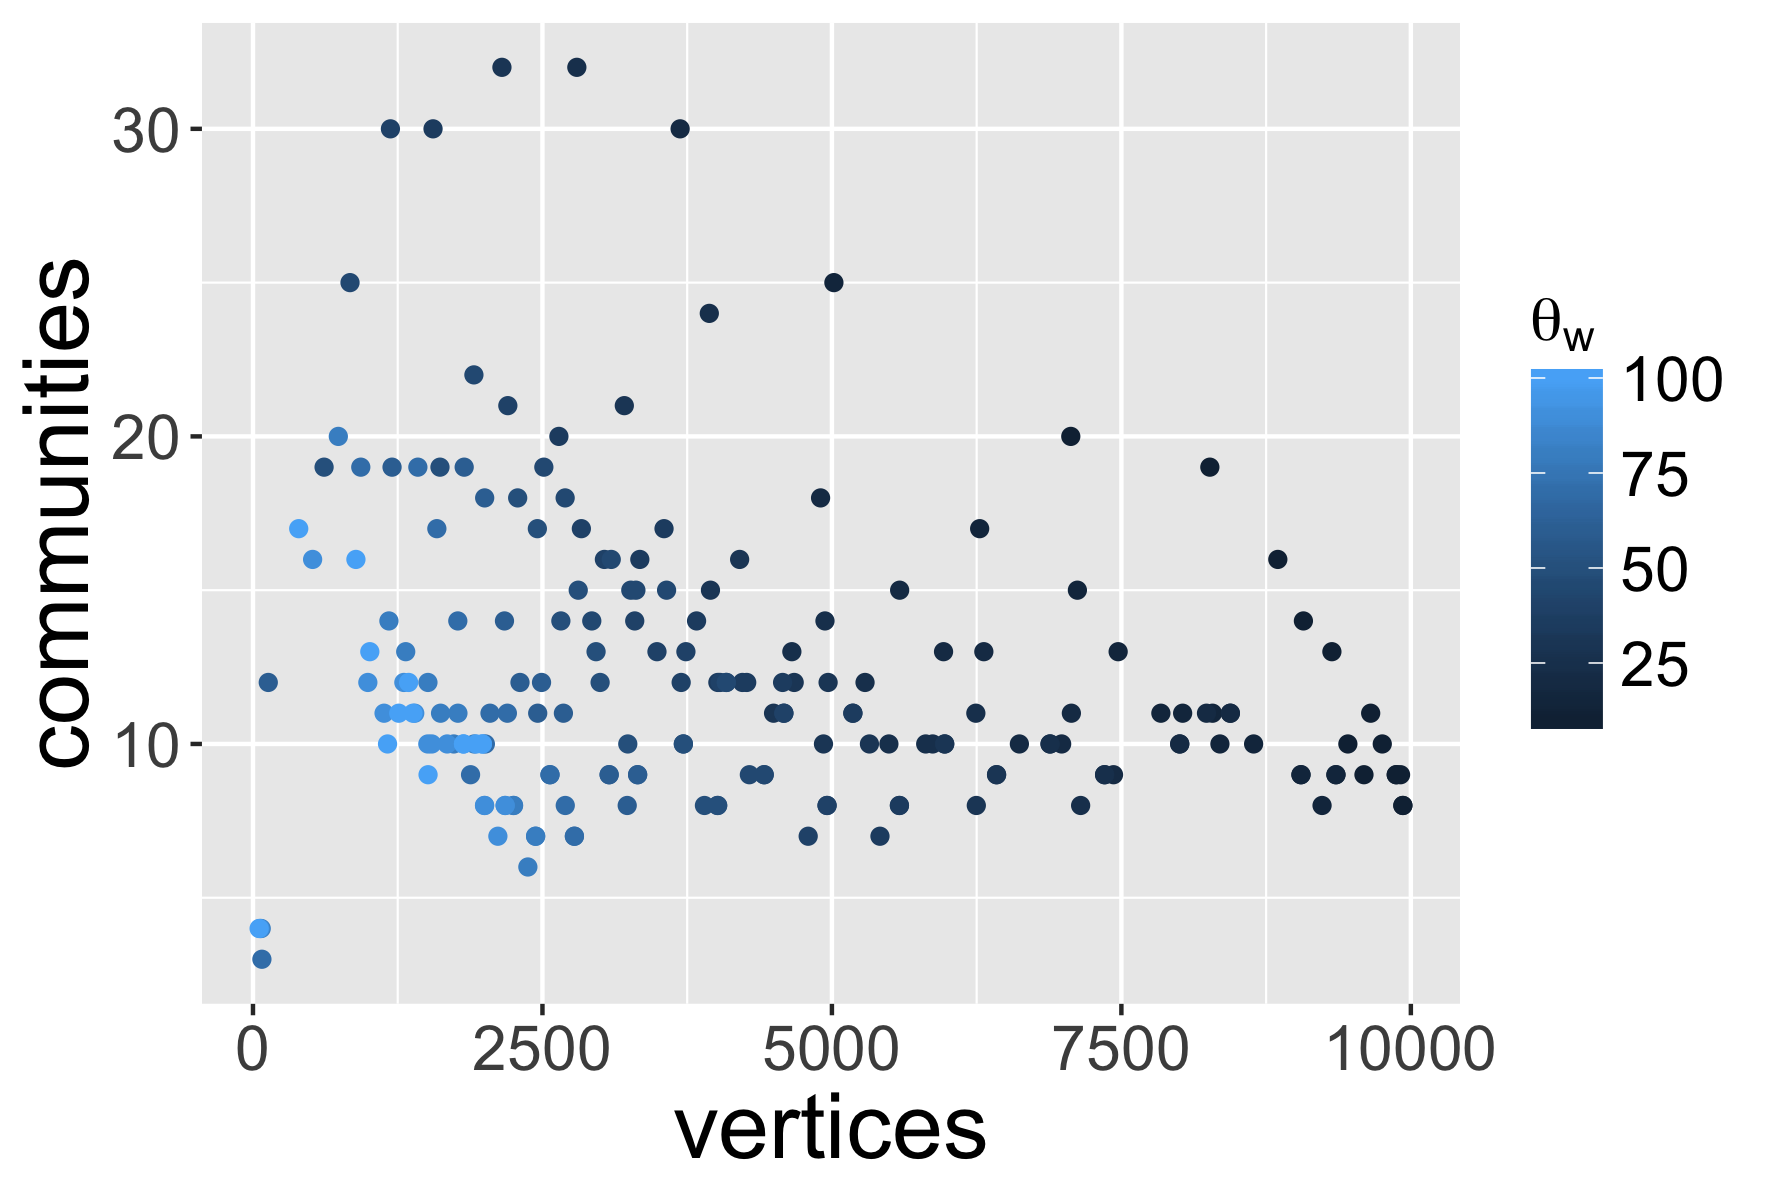
\includegraphics[width=0.49\linewidth]{Figures/Quantepistemo/pareto-com-vertices}
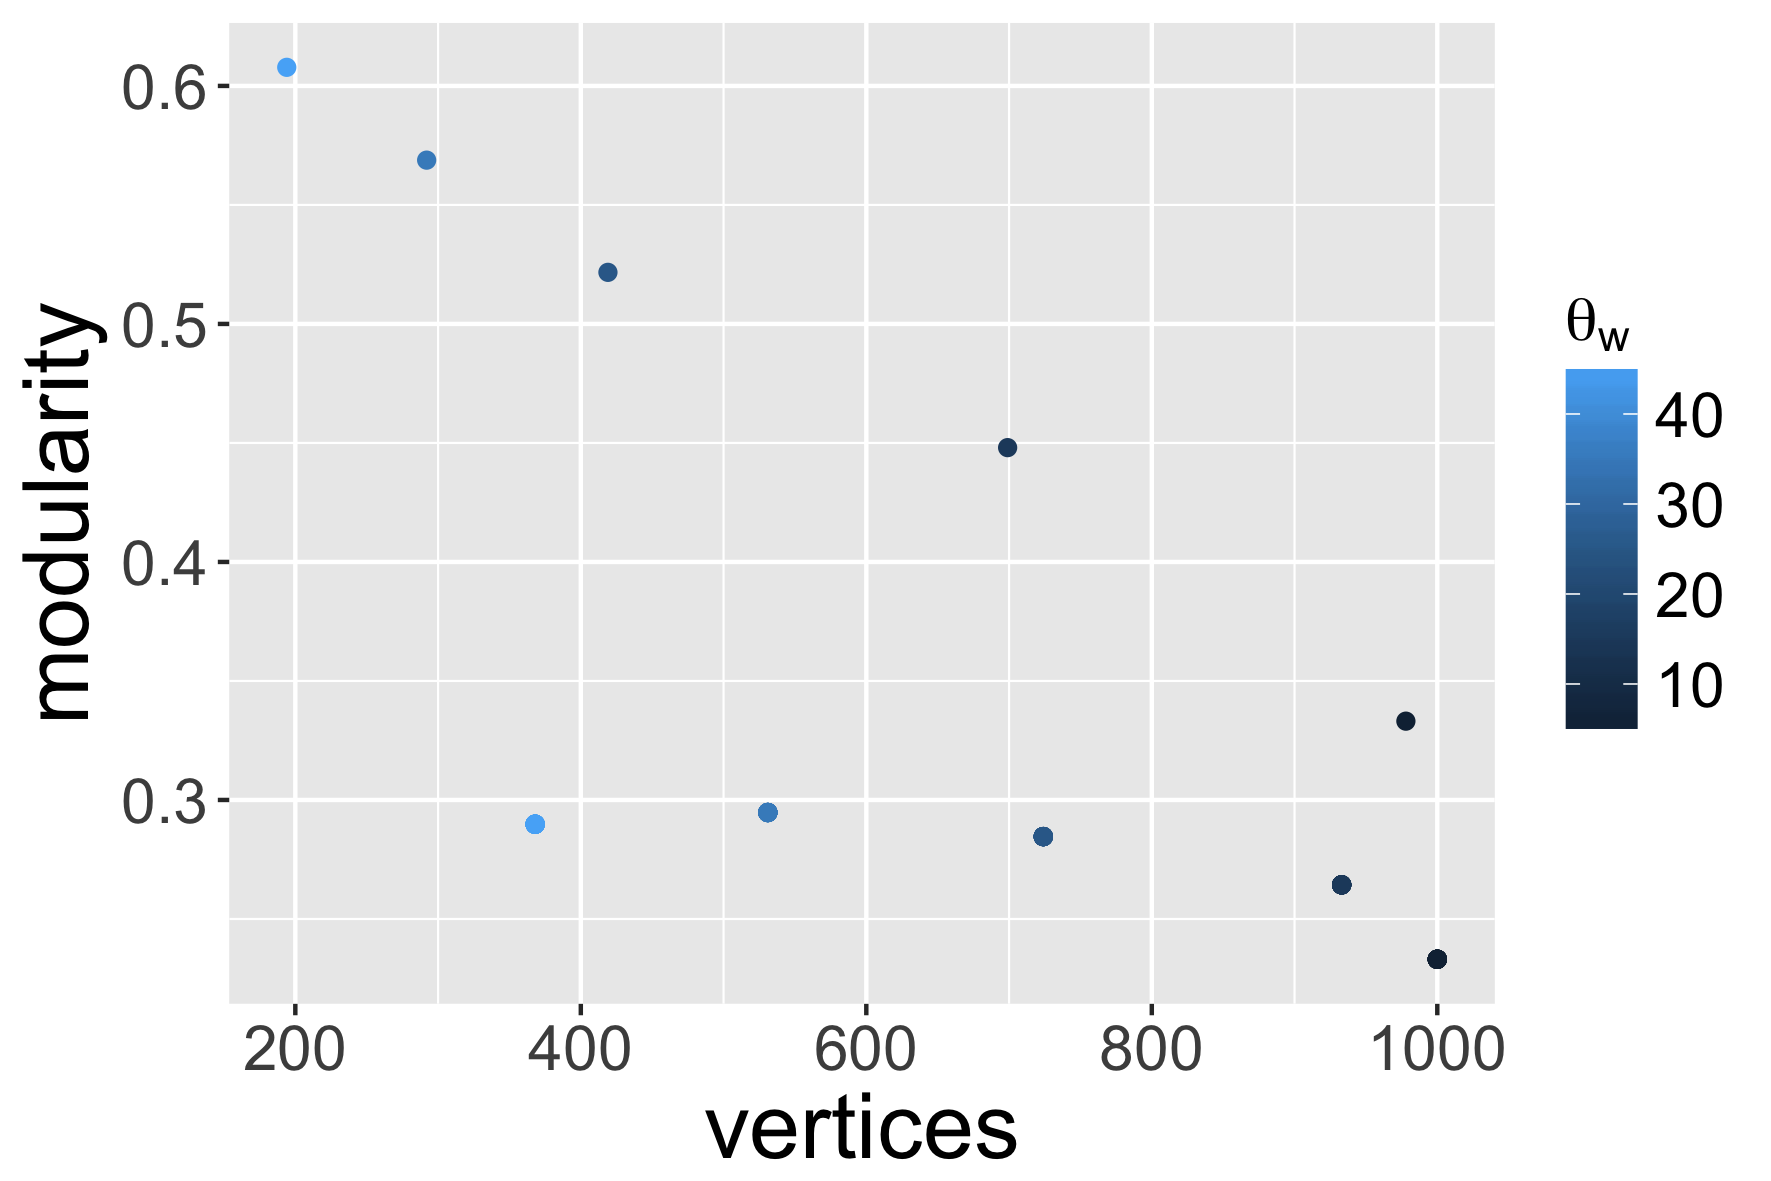
\includegraphics[width=0.49\linewidth]{Figures/Quantepistemo/pareto-modularity-vertices}\\
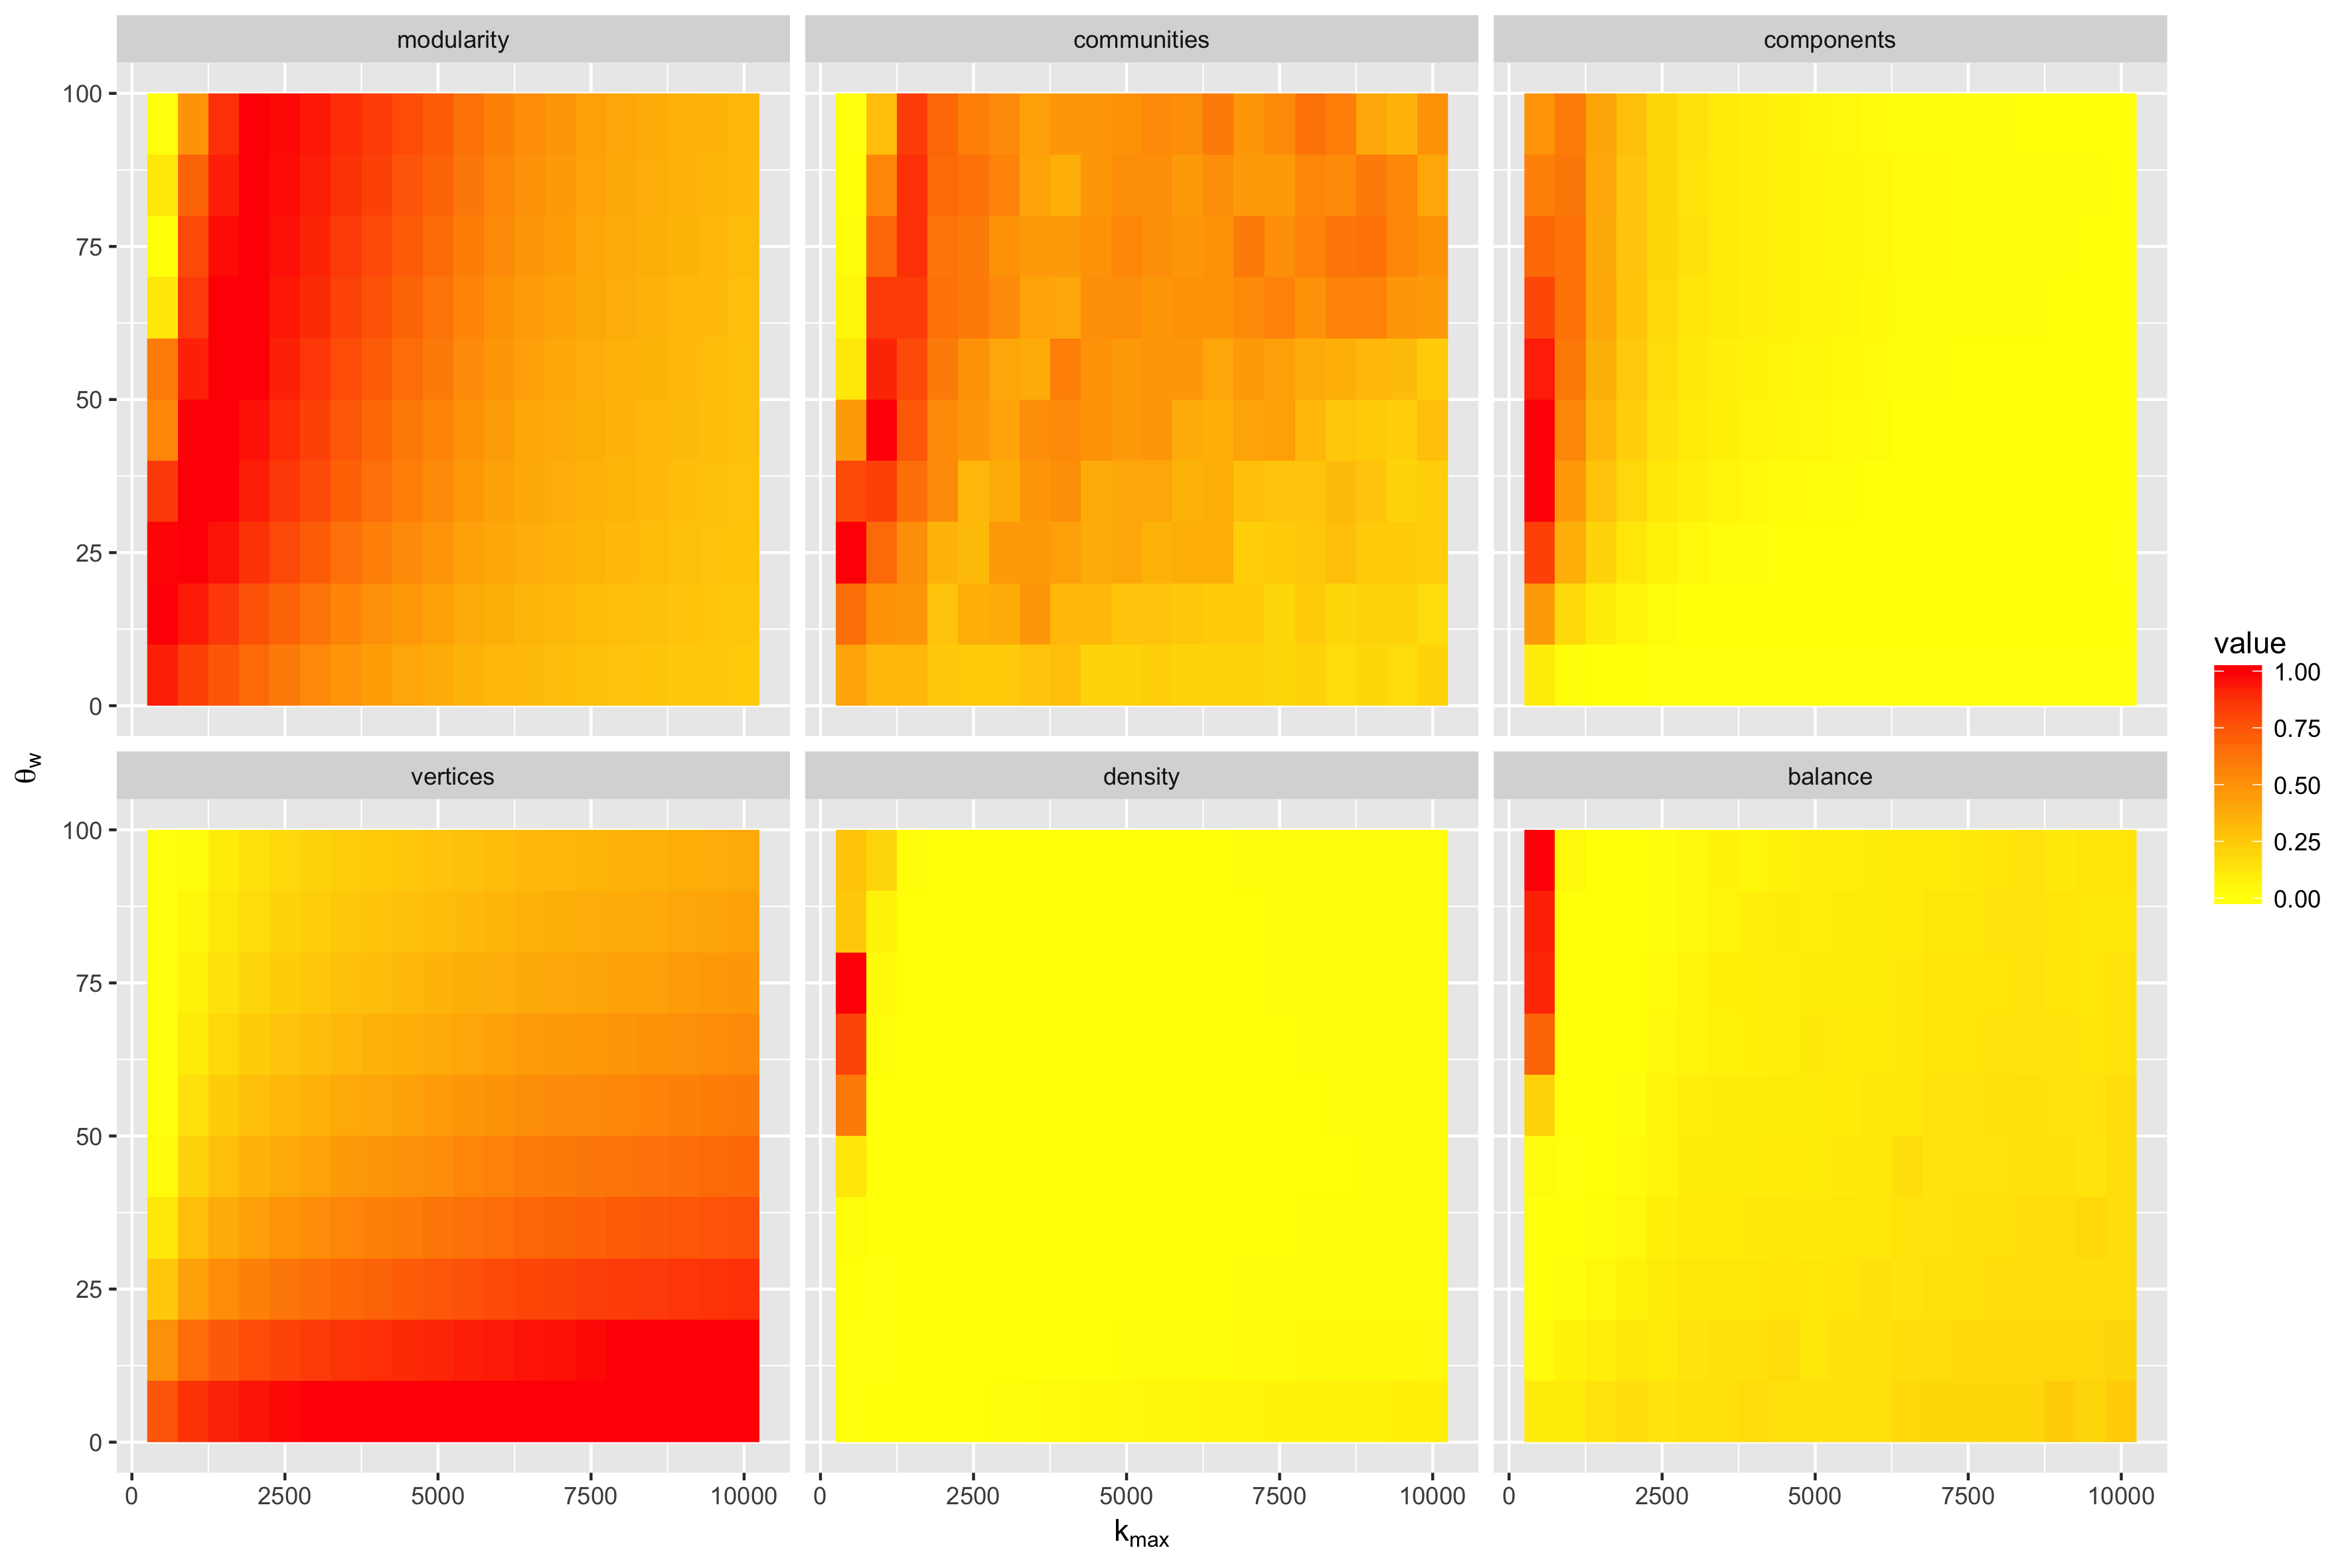
\includegraphics[width=\linewidth]{Figures/Quantepistemo/sensitivity_freqmin0_normalized}
\caption{Sensitivity analysis of network indicators to filtering parameters}{}
\label{fig:app:quantepistemo:sensitivity}
\end{figure}
%%%%%%%%%%%%%%%%%%



\paragraph{Semantic Network}{Réseau Sémantique}

% Visualisation du réseau sémantique.



%%%%%%%%%%%%%%%%%%
\begin{figure}
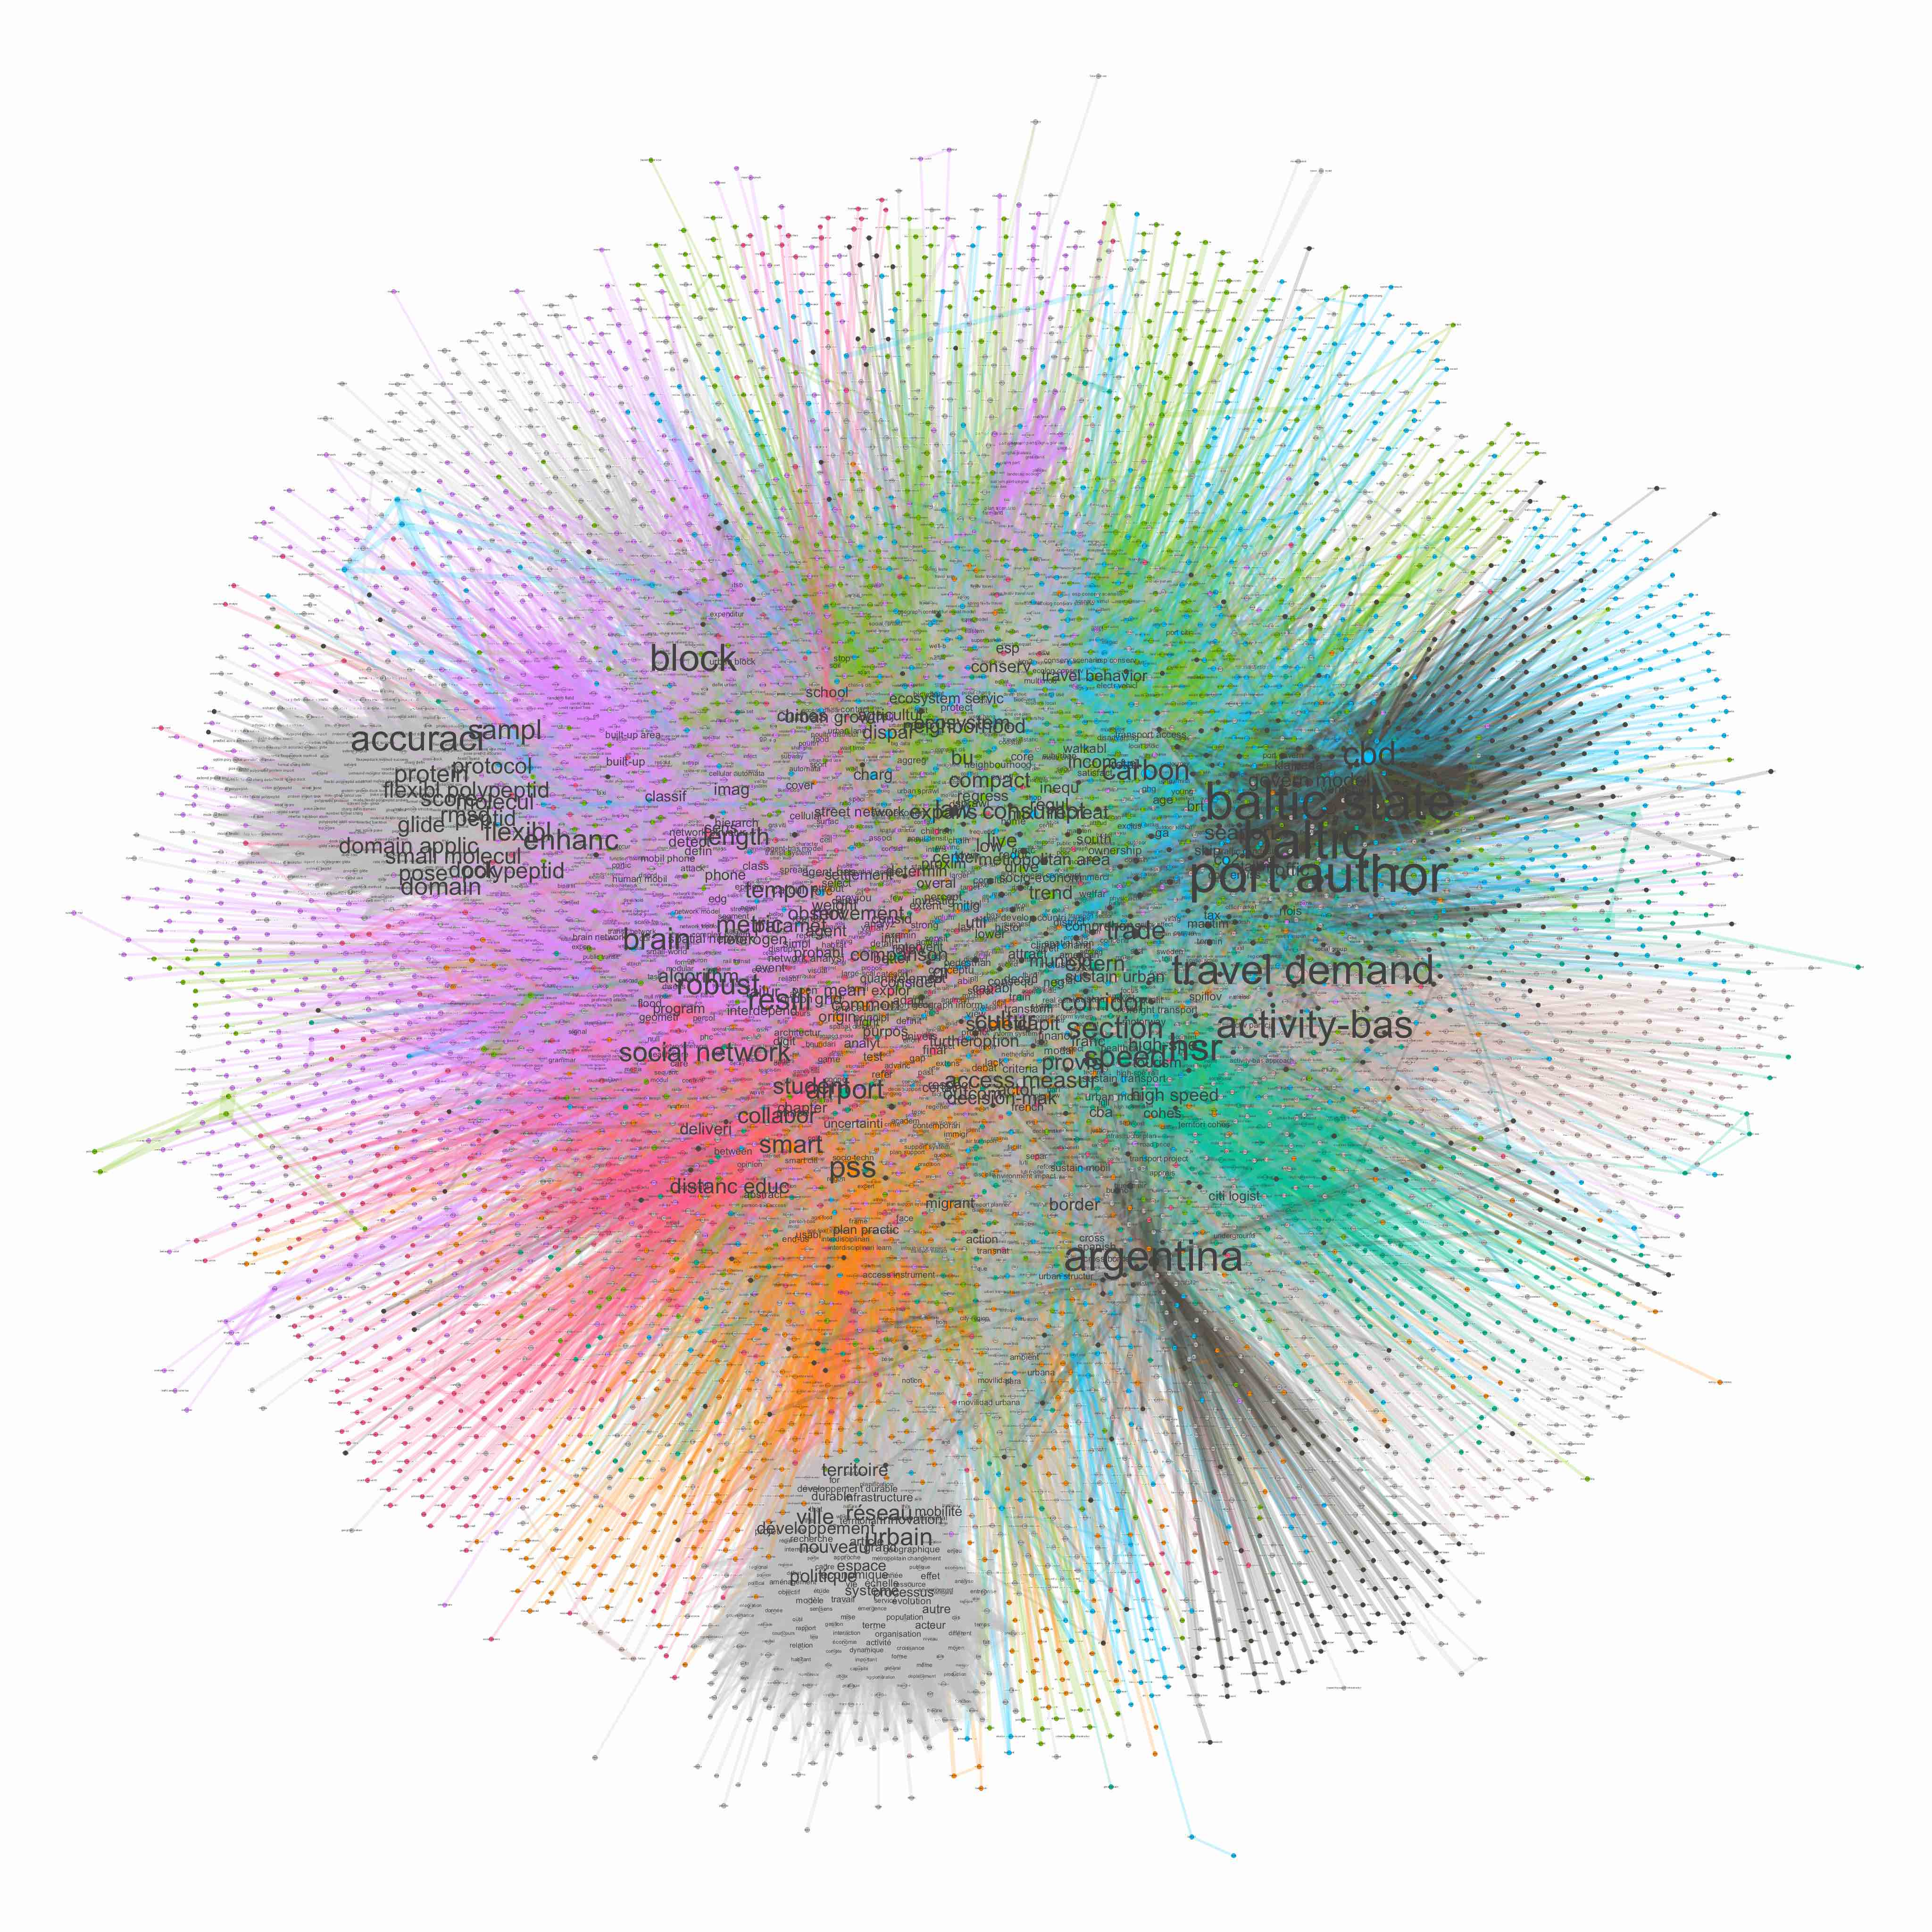
\includegraphics[width=\linewidth]{Figures/Quantepistemo/semantic}
\caption[Semantic network ][Réseau sémantique]{Semantic network of domains. Network is constructed by co-occurrences of most relevant keywords. Filtering parameters are here taken according to the multi-objective optimization done in Fig.~\ref{fig:sensitivity}, i.e. $(k_{max}=,e_{th}=,f_{min},f_{max}=)$. The graph spatialization algorithm (Fruchterman-Reingold), despite its stochastic and path-dependent character, unveils information. A zoomable vectorial file (\texttt{.svg}) of the network is available as Supplementary Material.}{}
\label{fig:quantepistemo:semanticnw}
\end{figure}
%%%%%%%%%%%%%%%%%%





\stars





%----------------------------------------------------------------------------------------

\newpage

%%%%%%%%%%%%%%%%%%%%%%%
\section{Modelography}{Modélographie}

\label{app:sec:modelography}


%----------------------------------------------------------------------------------------



\subsection{Systematic Review Methodology}{Méthodologie de la revue systématique}


Choix possible : extraire les mots-clés pertinents par sous-communautés du réseau de citations, puis prendre les plus pertinents ensuite.
ou (a priori ce que l'on fait) extraire sur le corpus complet, puis récupérer par sous-communautés. Pour un petit corpus, deuxième plus souhaitable, notion de pertinence moins importante que pour du big-data (mentionner Patents et Cybergeo, ressemblances et différences).




% random stuff removed manual screening 
%computer sci, neurosci, geology, chem/bio terrorism WTF ? , theoretical physics, eco des orgs, socio (aids ethiopia ?), target tracking, rice storage culinary qual, bulimic, smart cities, bullshit territorialité Die, chinese migrants !, chinese tourist HongKong, papier CN desakota (cité migrdyn), health, hydrology, paysage hautes corbières, musical implication network, finance capitalism, produit territoire pomme des alpes, mobilité sociale, vibration pont hsr, ontological knowledge industri., signal processing, anger/agression, flocks/schools, friendship and mobility, consumer brand,  aghion ? , colorectal cancer texas, lidar urban, mediteranean cities, sun and sand tourism, gender car use, gold rush movies, urban informatics, "best outside US", badger, robots beacon, milieux innovateurs, politique univ villes la rochelle etc, cosmology, economie de la qualité,  handbook adult resilience, stock price, archeo chefferie, speculative urb, Mendoza arg, subway platfrom ventilation, magaliths, crowding HK light rail !, terrritoire familiaux naples classes sup, performing arts series, sncf tunnel rig, china snow disaster; fabriq rue paris 19e, geopol inuit, espace public beyrouth, greenway., desire named streetcar, jeddah, french competitino rail myth, Equip the warrior instead of manning the equipment, aparheid namibia, baselIII finance, tokyo, espace transfrtontalier, transport proteins !, hedonic rail road noise, croissance syst urbain loi metropol, maritime nw indonesia, eco sociale au quebec, first world urban activism, hybrid.. , gentrif nvel urba, [before] Estimation of local spatial scale : otpicians !, stations de montange, street gang sptail pattern LA, SFI adress !, bogota BRT, transport noise, brussel urban geology, drosohiplia embryo






% hand classifications :
Journals $\rightarrow$ disciplines
jtgeo : geography, jtlu : transportation, transportation research, epb : geography\ldots

geography includes urbanisme, etudes urbaines si pas trop proche du planning (urban durable).









